\documentclass[class=report, crop=false]{standalone}
\usepackage[subpreambles=true]{standalone}

\begin{document}
    \section{Feedback}
    \label{Feedback}
    På de næste tre billeder kan man se den feedback som vi har fået fra opgave 3. Vi har som helhed ikke modtaget meget konstruktiv kritik, som derved gør det svært at forbedre vores rapport. 
    \begin{figure}[H]
        \centering
        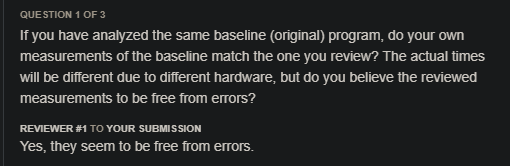
\includegraphics[width=\textwidth]{Spørgsmål1.png}
        \caption{Feedback på spørgsmål1.}
        \label{fig:Feedback1}
    \end{figure}

    \noindent Som set på billedet nedenfor får vi fortalt at vi ikke har nogle “fejl” I vores beregninger, som er positivt, men ikke giver noget vi kan arbejde videre på. 
    \begin{figure}[H]
        \centering
        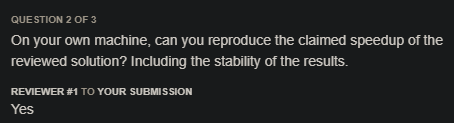
\includegraphics[width=\textwidth]{Spørgsmål2.png}
        \caption{Feedback på spørgsmål2.}
        \label{fig:Feedback2}
    \end{figure}
    
    \noindent På billede nedenfor får vi igen kort svar, havde vi fået at vide hvad for nogle resultater de fik af at køre vores program, kunne vi sammenligne og diskutere de to forskellige svar.
    \begin{figure}[H]
        \centering
        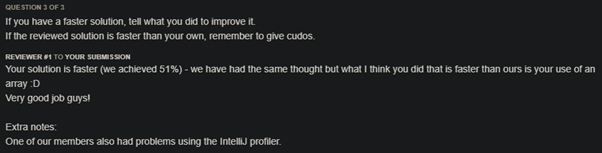
\includegraphics[width=\textwidth]{Spørgsmål3.png}
        \caption{Feedback på spørgsmål3.}
        \label{fig:Feedback3}
    \end{figure}

\end{document}